% This LaTeX was auto-generated from MATLAB code.
% To make changes, update the MATLAB code and export to LaTeX again.

\documentclass{article}

\usepackage[utf8]{inputenc}
\usepackage[T1]{fontenc}
\usepackage{lmodern}
\usepackage{graphicx}
\usepackage{color}
\usepackage{hyperref}
\usepackage{amsmath}
\usepackage{amsfonts}
\usepackage{epstopdf}
\usepackage[table]{xcolor}
\usepackage{matlab}
\usepackage[margin=2cm]{geometry}
% \geometry{top=1.5cm}
\sloppy
\epstopdfsetup{outdir=./}
\graphicspath{ {./ECE345_CQ03_images/} }

\begin{document}

\matlabtitle{ECE 345/ME 380: Introduction to Control Systems}

\matlabheading{Collaborative Quiz \#3}


\matlabheadingtwo{1.1 Location of poles and zeros of G(s)}

\begin{matlabcode}
num1=[1]; den1=[1 7 12 0];roots(den1)
\end{matlabcode}
\begin{matlaboutput}
ans = 3x1
     0
    -4
    -3
\end{matlaboutput}

\matlabheadingtwo{1.3 Step response of the open-loop system}

\begin{matlabcode}
sys1=tf(num1,den1)
\end{matlabcode}
\begin{matlaboutput}
sys1 =

          1
  ------------------
  s^3 + 7 s^2 + 12 s

Continuous-time transfer function.
\end{matlaboutput}
\begin{matlabcode}
step(sys1);grid;legend('G(s)','location','northwest')
\end{matlabcode}
\begin{center}
\includegraphics[width=\maxwidth{56.196688409433015em}]{figure_0.eps}
\end{center}

\matlabheadingtwo{2.5 Step response of the closed-loop system with K=100 over 0 to 20}

\begin{matlabcode}
K=100;tfinal=20;
sys2=K*feedback(sys1,K)
\end{matlabcode}
\begin{matlaboutput}
sys2 =

            100
  ------------------------
  s^3 + 7 s^2 + 12 s + 100

Continuous-time transfer function.
\end{matlaboutput}
\begin{matlabcode}
t=0:0.01:tfinal;
step(sys2,t);grid;legend('G_{CL}(s)','location','northwest');legend('G_{CL}(s)')
% legend called twice to fix subscript bug
\end{matlabcode}
\begin{center}
\includegraphics[width=\maxwidth{56.196688409433015em}]{figure_1.eps}
\end{center}

\end{document}
